\documentclass[12pt]{article}
\usepackage{rotating}
\usepackage[utf8]{inputenc}
\usepackage[T1]{fontenc}
\usepackage[ngerman]{babel}
\usepackage{here}
\usepackage{listings} 
\lstset{language=XML} 
\lstset{numbers=left, numberstyle=\tiny, numbersep=5pt} \lstset{language=Perl}
\usepackage{xcolor}
\usepackage{tikz}
\usepackage{tabularx}
\usepackage{booktabs, multicol, multirow}
\usepackage{rotating}
\usepackage{bigstrut}
\usepackage{svg}
\usepackage{wrapfig}
\usepackage{pdfpages} 
\usepackage{floatflt}
\usepackage{amsmath, amssymb}
\usepackage[printonlyused]{acronym} 
\usepackage{textcomp}

\lstdefinelanguage{JavaScript}{
	keywords={typeof, new, true, false, catch, function, return, null, catch, switch, var, if, in, while, do, else, case, break},
	keywordstyle=\color{blue}\bfseries,
	ndkeywords={class, export, boolean, throw, implements, import, this},
	ndkeywordstyle=\color{darkgray}\bfseries,
	identifierstyle=\color{black},
	sensitive=false,
	comment=[l]{//},
	morecomment=[s]{/*}{*/},
	commentstyle=\color{purple}\ttfamily,
	stringstyle=\color{red}\ttfamily,
	morestring=[b]',
	morestring=[b]",
	extendedchars=true,
	basicstyle=\footnotesize\ttfamily,
	showstringspaces=false,
	showspaces=false,
	numbers=left,
	numberstyle=\footnotesize,
	numbersep=9pt,
	tabsize=2,
	breaklines=true,
	showtabs=false,
	captionpos=b
}

\lstset{literate=%
	{Ö}{{\"O}}1
	{Ä}{{\"A}}1
	{Ü}{{\"U}}1
	{ß}{{\"ss}}1
	{ü}{{\"u}}1
	{ä}{{\"a}}1
	{ö}{{\"o}}1
	{~}{{\textasciitilde}}1
}

%\usepackage{hyperref}
\usetikzlibrary{arrows,shapes,snakes,automata,backgrounds,petri}
\lstdefinestyle{base}{
  language=xml,
  emptylines=1,
  breaklines=true,
  basicstyle=\ttfamily\color{black},
  moredelim=**[is][\color{red}]{@}{@},
}


\newcommand{\autorPraxisbericht}{Malte Möller}
\newcommand{\titelPraxisbericht}{Entwicklung und Pilotierung eines digitalisierten Zeiterfassungsprozesses für das Unternehmen COM Software GmbH}
\newcommand{\titelVeranstaltung}{{\sl Exposé}}
\newcommand{\ersterBetreuer}{Prof.\ Dr.\ Martin Przewloka}
\newcommand{\zweiterBetreuer}{Prof.\ Dr.\ rer.\ nat.\ Martin Rupp}
\newcommand{\dritterBetreuer}{Helmut Röse}
\newcommand{\vierterBetreuer}{Dennis Panz}
\newcommand{\abgabeortPraxisbericht}{Frankfurt am Main}
\newcommand{\datumAbgabePraxisbericht}{1.\ April 2017}


\usepackage[ngerman]{babel}
\usepackage{times}
\usepackage{natbib}
\usepackage{pdfpages}
\usepackage{amssymb}
\usepackage{amsmath}
\usepackage{graphicx}
\usepackage{svg}
\usepackage{eurosym}
\usepackage{txfonts}
\usepackage{pifont}
\usepackage{url}
\usepackage{colortbl}
\urlstyle{tt}
\usepackage{tikz}
\usepackage{pgflibrarysnakes}
\usetikzlibrary{shadows,fadings}
\usetikzlibrary{decorations}
\usetikzlibrary{arrows} % LATEX and plain TEX when using Tik Z


%\usepackage[paper=a4paper, 
%%outer=15mm, 
%%inner=30mm, 
%%top=40mm, 
%%bottom=25mm, 
%bindingoffset=10mm]{geometry} 



\definecolor{white}{gray}{1.00}
\definecolor{black}{gray}{0.00}
\definecolor{skyblue}{cmyk}{0.4, 0.2, 0.0, 0.0}             % HKS44-40
\definecolor{blue}{cmyk}{1.0, 0.5, 0.0, 0.0}                % HKS44-100
\definecolor{lightblue}{cmyk}{0.7, 0.35, 0.0, 0.0}          % HKS44-70
\definecolor{darkblue}{rgb}{0.04, 0.16, 0.32}               % 
\definecolor{extradarkblue}{cmyk}{1.00, 0.70, 0.10, 0.50}   % HKS41-100
\definecolor{darkgreen}{cmyk}{1.0, 0.0, 0.9, 0.2}           % HKS57-100
\definecolor{green}{cmyk}{0.65, 0.0, 1.0, 0.0}              % HKS65-100
\definecolor{purple}{cmyk}{0.5, 1.0, 0.0, 0.0}              % HKS33-100
\definecolor{indigo}{cmyk}{0.8, 0.9, 0.0, 0.0}              % HKS36-100
\definecolor{gray}{gray}{0.59}
\definecolor{lightgray}{gray}{0.4}
\definecolor{darkgray}{gray}{0.50}
\definecolor{darkcyan}{cmyk}{0.87, 0.4, 0.4, 0.0}
\definecolor{cyan}{cmyk}{0.78, 0.19, 0.01, 0.0}
\definecolor{lightcyan}{cmyk}{0.39, 0.095, 0.005, 0.0}
\definecolor{extralightcyan}{cmyk}{0.16, 0.1, 0.0, 0.0}
\definecolor{beetleBlue}{RGB}{64,80,127}

\usepackage[
colorlinks=false,
urlcolor=black,
linkcolor=black
]{hyperref}

\setlength{\textwidth}{15.5cm}     %
\setlength{\textheight}{23cm}      %
\setlength{\evensidemargin}{0cm} %
\setlength{\oddsidemargin}{0.95cm}  %
\setlength{\topmargin}{-1cm}       %
\setlength{\topskip}{0cm}          %
\setlength{\headheight}{11pt}      %



%\setlength{\textwidth}{15.5cm}     %
%\setlength{\textheight}{23cm}      %
%\setlength{\evensidemargin}{1.5cm} %
%\setlength{\oddsidemargin}{1.5cm}  %
%\setlength{\topmargin}{-1cm}       %
%\setlength{\topskip}{0cm}          %
%\setlength{\headheight}{11pt}      %


\title{%
	\titelPraxisbericht\\%
	\vspace{8mm}{\large Praxisbericht im Studiengang}\\%
	{\LARGE Bachelor Business Information Management}\\%
	{\large an der}\\%
	{\LARGE Provadis - School of International}\\%
	{\LARGE Management and Technology}\\%
}

\author{%
	{\normalsize vorgelegt von}\\%
	\vspace{4mm}\autorPraxisbericht\\%
	{\normalsize im Fach}\\
	{\LARGE \fach}\\
	\vspace{4mm}~\\{\normalsize Betreuer}\\%
	\ersterBetreuer}

\date{
	\vfill\abgabeortPraxisbericht, \datumAbgabePraxisbericht\\%
	~\\%
	
\includegraphics[scale=.75]{ComLogo.png}\hfil
	
\includegraphics[scale=.22]{ProvadisLogo.png}%
}


\newcommand{\Lab}[3] { %
 \put(#1,#2){\makebox(0,0){\shortstack[c]{#3}}}%
}

\newcommand{\lb}{\linebreak}%
\newcounter{wMinipage}%
\newcommand{\tiktxt}[4]{%
\setcounter{wMinipage}{#3*\real{1.3}}
\draw(#1 mm,#2 mm) node {\begin{minipage}{\thewMinipage mm}\begin{center}\setlength{\baselineskip}{2.5ex} #4\end{center}\end{minipage}};%
}%
\newcommand{\rtiktxt}[5]{%
\setcounter{wMinipage}{#3*\real{1.3}}
\draw(#1 mm,#2 mm) node[rotate=#5] {\begin{minipage}{\thewMinipage mm}\begin{center}\setlength{\baselineskip}{2.5ex} #4\end{center}\end{minipage}};%
}%





\newcommand{\spw}{StaffIT pro web}
\begin{document}

\maketitle
\thispagestyle{empty}

\newpage
\pagestyle{headings}


\input{./Abschnitte/Erklärungen.tex}

\pagestyle{headings}

\newpage
\section*{}
	\tableofcontents
\newpage
\addcontentsline{toc}{section}{Abbildungsverzeichnis}
\listoffigures
\newpage
\addcontentsline{toc}{section}{Tabellenverzeichnis}
\listoftables
\addcontentsline{toc}{section}{Listing-Verzeichnis}
\lstlistoflistings

\newpage
\input{./Abkürzungsverzeichnis.tex}

\newpage
\pagenumbering{arabic}
\setcounter{page}{1}

\section{Einleitung}
Jede Organisation nutzt gewisse Prozesse um den betrieblichen Alltag und das dazugehörige Geschäft abzuwickeln. Diese Prozesse können in den unterschiedlichsten Formen abgebildet sein. Zum einen können die Prozesse einfach nur nach bestem Wissen und Gewissen gelebt werden, ganz nach dem Motto \flqq so wie es schon immer war\frqq. Eine erste Ausbaustufe ist der dokumentierte Prozess. Es ist also beschrieben, wie der jeweilige Ablauf normalerweise ausgestaltet sein soll. Im Optimalfall wurde dieser sogar schon analysiert und zu dem bestmöglichen Prozess optimiert. Doch reicht das für einen erfolgreichen Betrieb oder Bedarf es hier weiterer Aktionen?
\subsection{Erläuterung}
Es gibt immer Wege und Möglichkeiten etwas zu Verbessern. Mit dem Zeitalter der Digitalisierung sind unterstützende Software-Lösungen meist der Schlüssel zur Optimierung. Auf Prozesse bezogen kann dies beispielsweise die Softwareunterstützung einiger Teilaufgaben sein, oder sogar die gesamte Digitalisierung aller Prozessschritte in einem System. Um allerdings ein solches zu implementieren, sind wiederum Informationen von und für andere Systeme von großer Relevanz. Es müssen Schnittstellen erstellt und integriert werden. Um dies zu gewährleisten, muss der IST-Zustand mit den damit verbundenen Problemstellungen detailliert definiert sein. Diese Arbeit soll den IST-Prozess der Arbeitszeiterfassung im Gesamtkonzept eingliedern und bestmöglich beschreiben. Nach anschließender Analyse kann die Entwicklung eines Prototypen starten. 
\subsection{Betrieblicher Kontext} \label{betrieb}
Die \textit{COM Software GmbH} ist ein mittelständischer IT-Dienstleister mit Sitz im Rhein-Main-Gebiet. Der Branchenfokus der europaweiten Kunden liegt bei Banken und Finanzdienstleistern beziehungsweise deren teilweise ausgegliederten Rechenzentren und IT-Sparten. \\
Das Unternehmen wurde im Jahr 1996 als GmbH von zwei Gesellschaftern gegründet und wird von Herrn Helmut Röse geleitet. Es werden 2017 zum Jahresende 130 Mitarbeiter beschäftigt, davon ein Teil festangestellt und ein Teil freiberuflich. \\
Die Schwerpunkte der Beratungstätigkeit liegen bei der Softwareentwicklung und System\-administration sowie der Konzeption und Implementierung von individuellen Softwarearchitekturen. Abgerundet wird das Portfolio durch ein Angebot von Lösungen im Bereich der Beratungsleistung zur zielgerichteten Informationsversorgung von Organisationseinheiten im Rahmen von Data-Warehouse und Business-Intelligence. \\
Im Bereich der Digitalisierung ist die COM Software GmbH mit Sicherheit am Puls der Zeit, da viel Wert auf aktuelles Wissen gelegt wird. In den Bereichen Geschäftsprozessmanagement und Dokumentenmanagement sind bereits Systeme implementiert. Einige Prozesse, wie beispielsweise der Onboarding Prozess sind modelliert, in die Organisation integriert und werden gelebt. 
\subsection{Sensibilisierung des Themas}
Auch bei der COM Software GmbH gibt es ein hohes Maß an Optimierungspotential. Eine Prozesslandkarte ist erstellt, auf welcher die unterschiedlichsten betrieblichen Prozesse abgebildet sind. Einer dieser Prozesse ist die Arbeitszeiterfassung, welche in direktem Zusammenhang zu dem Rechnungslegungsprozess steht. Jeder Berater welcher im Kundenprojekt tätig ist, muss am Ende eines jeden Monats für seine Projekte Daten bei der COM Software GmbH für die Stundenabrechnung einreichen. Die Kerninformationen spiegeln sich in zwei Dokumenten, dem Stundennachweis und der Beraterrechnung wieder. Diese Dokumente werden zum aktuellen Zeitpunkt per Post oder Mail zur COM Software GmbH gesendet. Identifiziertes Problem ist, dass dieser Dateneingang kein einheitlichen Kommunikationsweg und kein einheitliches Format besitzt. Deshalb ist auch die einheitliche Weiterverarbeitung mit Systemunterstürzung ohne große manuellen Tätigkeiten unmöglich. Genau dieses Problem soll durch die Standardisierung und Digitalisierung des Informationseingangs mithilfe einer Applikation gelöst werden.
\subsection{Ziel der Arbeit}
Das Projekt hat ein klar definiertes Ziel. Es soll ein testfähiger Prototyp entstehen, welcher alle relevanten Daten für die Weiterverarbeitung in einem System konsolidiert. Jeder Berater soll die Informationen auf der einheitlichen Plattform eintragen. Eine hohe User Akzeptanz muss durch die Applikation sichergestellt werden. Deshalb sollen Grundinformationen von vornherein geladen und dem Nutzer zur Verfügung gestellt werden. Durch Schnittstellen zu Fremdsystemen sollen personalisierte Auswahlmöglichkeiten vorkonfiguriert und der gesamte Informationsgehalt aufbereitet werden. Durch Kennzahlen soll der IST-Prozess mit dem optimierten Prozess verglichen werden. 
\subsection{Aufbau der Arbeit}
Bei dem in Absatz \ref{betrieb} beschriebenen Onboarding Prozess ist schon ein spürbarer Mehrwert gegenüber der ursprünglichen Checkliste in Form eines Blatt Papiers zu erkennen. \\
Um den Prozess der Arbeitszeiterfassung und Verarbeitung zu Digitalisieren, wird der Inhalt dieser Arbeit in mehrere Stufen untergliedert. Zum Einen soll eine breite Grundlagenforschung und entsprechende Statistiken den aktuellen Stand der Digitalisierung, insbesondere in Bezug auf Geschäftsprozessmanagement und Dokumentenmanagement, darlegen. \\
Im nächsten Schritt soll der Ist-Prozess erhoben, bewertet und der optimierte Soll-Prozess entwickelt werden. Ist der Prozess final modelliert und mit dem Kunden abgestimmt, geht es in die Umsetzungsphase um einen Piloten zu entwickeln. In diesem konkreten Prozess gilt die Fachabteilung der Abrechnung als Kunde und wird in ständigem Austausch die Qualität der Lösung bestätigen. \\
Während der Umsetzung muss die Frage der richtigen Technologie anhand methodischer Analyse geklärt werden. Wichtig sind hier besonders die Aspekte Datensicherheit und Zugriffsschutz, da es sich um sensible Personenbezogene Daten handelt. \\
Abschließend wird der Pilot mit Kennzahlen, wie zum Beispiel den Prozesskosten und der Durchlaufzeit bewertet. Hierfür wird die Fachseite sowohl den Ist-Zustand als auch den Soll-Zustand nach erfolgreicher Implementierung der Lösung in Bezug auf die benötigten Ressourcen messen.
\subsection{Forschungsmethode}
Die Grundlage für ein erfolgreiches Projekt ist die korrekte und vor allem vollständige Aufnahme der IST-Situation. Nur anhand dieser kann ein hohes Optimierungsmaß erreicht werden. Sobald der IST-Zustand methodisch aufgenommen ist, wird dieser Analysiert und der SOLL-Zustand modelliert. Das Ergebnis soll anschließend in Form eines Prototypen entwickelt und vertestet werden.   



\section{Grundlagen zur Bearbeitung}
Für das Projektverständnis sind Grundlagen zu schaffen. Sowohl die Einordnung des Projektthemas
als auch die unterschiedlichen Tools, Informationssysteme und genutzten Methoden müssen verständlich erläutert sein, um den Gesamtkontext der Arbeit einordnen zu können.

\subsection{Inbound Marketing}
Inbound Marketing ist eine Art des Marketings, die auf personalisierter Werbung besteht und den Kunden zum Unternehmen bringen soll. Der Kunde soll, der Firma gegenüber, loyal und freundlich gesinnt sein. Dies wird durch personalisierte Werbung erreicht, bei welcher der Kunde nicht direkt vom Marketing Team angesprochen wird. Dafür werden Kundendaten benötigt, mit welchen die Firma gezielt Werbung schalten kann. Diese Werbung wird nicht nur auf der eigenen Plattform betrieben, sondern erreicht den Kunden über mehrere Kanäle. Somit bleibt das Unternehmen dem Kunden im Hinterkopf und wenn sich ein Problem entwickelt, bei welchem das Unternehmen eine Lösung anbietet wird sich der Kunde an das  Unternehmen wenden.
\newline 
Allerdings spielt nicht nur Werbung eine große Rolle im Inbound Marketing, da die potenziellen Kunden erst einmal auf das Unternehmen aufmerksam werden müssen. Dies geschieht durch gute Erfahrungen von Bekannten oder Kollegen, genauso wie die Vorstellung der eigenen Leistungen. Dies kann durch die eigene Website sein, Soziale Medien oder Blogs, welche vom Marketing Team gepflegt werden. Wird der potenzielle Kunde durch solche Informationen auf das Unternehmen aufmerksam, kann sich, über Cookies oder ähnliches, das Unternehmen den User merken und ihm gezielt Werbung schalten. Somit bleibt das Unternehmen im Gedächtnis des potenziellen Kunden und sobald dieser eine Leistung benötigt, welche das besagte Unternehmen anbietet, wird er an dieses denken und sich an das Unternehmen wenden. Genauso ist es wichtig bei Suchmaschinen wie 'Google', 'Bing' etc. weit oben zu sein. Dadurch kann der potenzielle Neukunde das Unternehmen schneller entdecken. Des Weiteren besuchen die wenigsten Menschen die zweite oder dritte Seite einer Suchmaschine, weshalb es sehr von Vorteil für ein Unternehmen ist, bei Suchmaschinen weit oben gelistet zu sein.
\newline 
Ein weiterer Teil des Inbound Marketings ist es nicht alle Informationen auf einmal Preis zu geben. Besucht ein potenzieller Kunde eine Website, so kann er meist alle Informationen einsehen. Beim Inbound Marketing wird dem potenziellen Kunden nur ein Bruchteil der möglichen Informationen geliefert. Um an weitere zu kommen ist es notwendig eine Mail Adresse oder andere Daten, welche das Unternehmen weiter für Werbung nutzen kann, zu hinterlegen. Somit kann sich der Kunde weiter informieren und zeigt sein ehrliches Interesse an dem Unternehmen und das Unternehmen erhält nötige Daten, welche für weitere Inbound Marketing Strategien genutzt werden kann. 
\newline 
Damit die Werbung richtig personalisiert werden kann ist es wichtig für das Unternehmen, dass es seine Zielkunden kennt. Hierfür werden 'Buyers Personas' und 'Ideal Customer Profile' angelegt. 
\newline 
Um ein 'Ideal Customer Profil' anzulegen, muss ein Unternehmen wissen, wie die eigenen Kunden ausschauen. Sind es andere Unternehmen, so sollte klar sein, wie viele Angestellte die Kunden im Durchschnitt haben, welches Budget ihnen zur Verfügung steht, wo die Sitze des Unternehmens liegen und wie lange die Projekte oder einzelnen Geschäftsbeziehungen im durchschnitt dauern. Mit Hilfe dieses 'Ideal Customer Profil' können Unternehmen ermitteln, ob ein potenzieller Kunde in das Schema des Unternehmens passt oder ob es die eigene Kapazität übersteigt. Außerdem kann mit dem 'Ideal Customer Profil' ermittelt werden, auf welchen Plattformen die Kunden am besten zu erreichen sind, da große Unternehmen anders operieren, als Mittelständige oder Kleinunternehmen. 
\newline 
Bei den 'Buyers Personas' wird geschaut, wer dafür Zuständig ist die Geschäfte mit der eigenen Firma abzuwickeln. Dabei wird festgestellt, ob es ein Abteilungsleiter oder CEO des Unternehmens ist. Des weiteren wird geschaut, worauf die einzelnen Kunden achten. Dabei werden die bestehenden Kunden analysiert, um festzustellen, wo Gemeinsamkeiten bestehen und inwiefern sich die einzelnen Kunden unterscheiden. Anhand dieser Informationen wird festgestellt, welche Herausforderungen die einzelnen Kunden mit sich bringen und wie diese spezifisch in der Werbung angesprochen werden können, um das eigene Angebot attraktiv zu machen. 
\newline 
Mit Hilfe der Buyers Personas' und 'Ideal Customer Profile', kann das Unternehmen beginnen die eigenen Kunden in Gruppen zu unterteilen. Zu diesen Gruppen werden die potenziellen Neukunden ebenfalls zugewiesen, um die Werbung so individuell und attraktiv wie möglich zu gestalten. Somit kann viel mehr auf die eigenen Interessen der verschiedenen Kunden und Neukunden eingegangen werden. Die bestehenden Kunden haben das Gefühl, dass das Unternehmen genau weiß, was die Kunden brauchen und die möglichen Neukunden zeigen schneller Interesse, da gleich auf die eigenen Probleme und Bedürfnisse eingegangen wird. Sie denken gleich, dass das Unternehmen genau das bieten kann was sie benötigen. 
\newline 
Durch das Inbound Marketing lassen sich gute, lukrative und lange Geschäftsbeziehungen erstellen. Außerdem kann sich das Unternehmen viel besser selbst einschätzen und auch besser auf die Probleme und Herausforderungen der Kunden eingehen. Allerdings kostet Inbound Marketing viel Aufwand als gewöhnliche Marketing Methoden. Es muss spezifisch auf die Kunden eingegangen werden und die Kommunikation zwischen Unternehmen und Kunde steht im Vordergrund, weshalb die Unternehmen um einiges mehr an Arbeit in die Kundenbeziehungen stecken müssen. Seien es die bestehenden Kunden, welche nicht verloren gehen dürfen oder die Neukunden, welche über das Unternehmen selbst informiert werden müssen. Dennoch stechen die positiven Aspekte des Inbound Marketings deutlich heraus und viele Unternehmen, besonders Mittelständige und Start-Up Unternehmen nutzen diese Methode des Marketings um auf sich aufmerksam zu machen.

\subsection{Outbound Marketing}
Unter den Begriff Outbound Marketing fällt fast alles was zu den traditionellen Marketing Methoden zählt. Hier kommt der Kunde nicht zur Firma, sondern die Firma zum Kunden. 
\newline 
Die meisten Methoden des Outbound Marketings sind die bekannten Werbemethoden. Dazu zählen Spam, Kaltakquise, Briefpost, Radiowerbung, TV-Werbung, Flyer oder Vertreter. 
\begin{figure} [H]
	\centering
	\begin{minipage}[b]{.45\linewidth}
		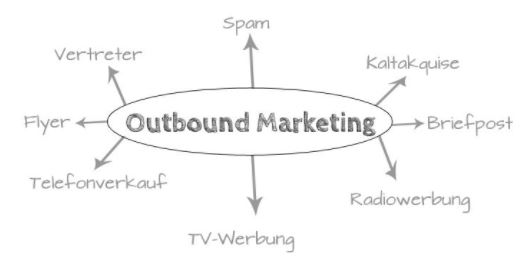
\includegraphics[width=7.5cm]{./Grafiken2/Outbound_Marketing.JPG}
		\caption{Outbound Marketing (/onlinemarketing.de/lexikon/outbound-marketing)}
		\label{Create_Zubereitung}
	\end{minipage}
\end{figure}
Alle diese Methoden haben gemeinsam, dass das Unternehmen sich an den Kunden wendet. Es wird immer eine große Anzahl an Leuten erreicht, jedoch gibt es meist nur wenige die sich überhaupt dafür interessieren, den Beruf ausüben oder Wissen in dem Bereich des Unternehmens haben. Die Strategie hinter diesen Methoden liegt darin, so viele Menschen wie möglich zu erreichen, damit die wenigen welche an dem Produkt interessiert sein könnten ebenfalls die Werbung erhalten. Genauso könnte das Interesse weniger Menschen oder Unternehmen durch diese Methode des Marketings geweckt werden, damit diese das Produkt oder die Dienstleistung des Unternehmens für sich in Anspruch nehmen. 
\newline
Somit gestaltet sich die Neukundenakquise mit Outbound Marketing etwas schwierig, da alle Methoden das Problem haben, zu viele Menschen zu erreichen, die höchstwahrscheinlich nie Kunden werden. Des weiteren kostet es sehr viel Arbeit und Geld, um genug Menschen zu erreichen, damit die richtige Person, die das Produkt oder die Dienstleistung kauft, dabei ist.
\newline 
Eine weitere Methode des Outbound Marketings sind Newsletter oder gezielte Mails an Kunden. Dabei wendet sich das Unternehmen ebenfalls an die Kunden, jedoch in einem viel kleineren Spektrum. Hierbei werden nur Kunden, die auch wirklich an der Dienstleistung oder dem Produkt interessiert sein könnten, diese erhalten. Newsletter müssen abonniert werden und nur wenn ein Account erstellt oder etwas von einer Website gekauft wurde, liegen die entsprechenden Daten vor, damit der Kunde diesen Newsletter erhält. Wurde die Option des Newsletters nicht ausgewählt können und düfren die Kunden diesen nicht erhalten, somit wendet sich das Unternehmen mit dieser Methode meist nur an bereits bestehende oder ehemalige Kunden. 

\subsection{Web Scraping}
Das Web Scraping ist ein Verfahren, welches genutzt wird, um Daten von verschiedenen Websites zu erhalten. Üblicherweise ist es ein automatisierter Prozess, welcher von Computerprogrammen ausgeführt wird. Dabei liest das Programm den Quelltext der gewünschten Website aus und speichert alle erwünschten und gesuchten Daten in einer Datenbank oder Tabelle ab.
\newline
Um dies zu erreichen muss das Programm die URL der Website, die ausgelesen werden soll, kennen. Daraufhin greift das Programm auf den Quelltext zu und liest diesen aus. Sollten Stichwörter auftauchen, die Adressen oder andere personenbezogene Daten suggerieren, werden diese oder die darauf folgenden Zeilen kopiert und in eine Datenbank gespeichert. Telefonnummern, E-Mail Adressen, Adressen und Kontaktdaten haben meist einen speziellen Aufbau, weshalb diese anhand dessen kopiert und gespeichert werden können. E-Mail Adressen beinhalten das '@' Zeichen und Telefonnummern eine Vorwahl. Daran können diese leicht vom Programm identifiziert werden.
\newline
Im Inbound Marketing kann Webscraping genutzt werden, um an die Daten der Kunden zu gelangen, welche erreicht werden sollen oder genügend Interesse gezeigt haben. Web Scraping wird meist zur Neukundenakquise eingesetzt, damit die entsprechenden Kunden diret kontaktiert werden können. Des Weiteren können so Nachforschungen angestellt werden, ob das anzuwerbende Unternehmen überhaupt in das eigene Kundenschema passt. 

\subsection{Data Wrangling}
Unternehmen, die Daten sammeln erhalten diese erst einmal in roher Form. Das bedeutet, dass diese Daten nicht sortiert und geordnet sind. Hierbei hilft das 'Data Wrangling'. Beim 'Data Wrangling' werden die gesammelten Daten genormt. Das Ziel dabei ist Daten,  die aus verschiedensten Quellen kommen, vergleichen zu können. Data Analysten verbringen etwa 70\% - 80\% ihrer Zeit damit die gesammelten Daten zu Normen. Dabei wird geschaut, wie viel Wert die unterschiedlichen Daten für das Unternehmen oder die Analyse hat. Als Nächstes werden die Daten aufgesplittet. Hierbei können aus einer Zeile in der Datenbank gleich mehrere werden. Da manche Daten einfacher zu vergleichen und analysieren sind, wenn sie getrennt werden. 
\newline
'Data Wrangling' ist eine Anstrengende und sehr repetitive Aufgabe. Es wird in 6 unterschiedliche Schritte unterteilt. Der erste Schritt ist die Entdeckung der Daten. Dabei wird herausgefunden, um was für eine Art Daten es sich handelt. Genauso machen sich die Data Analysten in diesem Schritt vertraut mit den Daten.
\newline
Im nächsten Schritt, dem 'Data Structuring', werden die Daten umstrukturiert. Dies muss gemacht werden, da die einzelnen Datensätze meist komplett unterschiedlich sind. Das kann daher kommen, dass die Daten aus unterschiedlichen Quellen stammen oder verschiedene Informationen enthalten. Damit mit den einzelnen Daten gearbeitet werden kann und diese auch miteinander verglichen werden können.
\newline 
Der dritte Schritt nennt sich 'Data Cleaning'. Hier geht es darum Fehler, die beim Importieren aufgetreten sind zu bereinigen oder schlechte Datensätze zu löschen. 
\newline 
Beim 'Data Enriching', dem vierten Schritt, wird sich die Frage gestellt, ob die vorhandenen Daten verschönert oder vermehrt werden müssen.
\newline
Im nächsten Schritt, namens 'Data Validating', kommen Qualitätsprobleme der einzelnen Datensätze zum Vorschein. Dabei wird die Richtigkeit sowie die Authentizität der Datensätze überprüft.
\newline
Das 'Data Publishing' ist der letzte Schritt und hierbei werden die Daten weiter verschoben, damit sie analytisch verarbeitet werden können. 

\input{./Abschnitte/Ist-Zustand.tex}


\input{./Abschnitte/Technologie.tex}

\input{./Abschnitte/prototyp.tex}

\newpage
\section{Fazit}
Dieses Kapitel reflektiert das durchgeführte Projekt. Die einzelnen Schritte werden in der Zusammenfassung chronologisch widergespiegelt. Die gewonnenen Ergebnisse für künftige Projekte und vor allem für das Management werden detailliert beschrieben. Der Ausblick bildet den Abschluss der Arbeit. Hier wird das geplante weitere Vorgehen beschrieben. Der Prototyp soll weiterentwickelt und anschließend für den produktiven Einsatz in das Unternehmen integriert werden.
\subsection{Zusammenfassung}
Das Management der COM Software GmbH hat in alle Bereiche des Unternehmens entsprechenden Einblick. Optimierungsmöglichkeiten sind vorhanden. Diese werden in internen Absprachen priorisiert. Anschließend fällt eine Einordnung und die jeweilige Projektentscheidung. So wurde die Thematik der Leistungsnachweise der im Projekt befindlichen Berater in diesen Plan aufgenommen und das Projekt aufgestellt.\\
Mit dem Projektstart wurden erste Termine mit der Fachabteilung abgestimmt, um die Thematik einzuordnen. Zu Beginn ist man von der reinen Arbeitszeiterfassung ausgegangen. Bereits in dem ersten Termin wurde deutlich, dass dies als Anforderung nicht ausreicht und die Thematik in einem größeren Kontext betrachtet werden muss. Somit startete die in Abschnitt \ref{IstProzess} beschriebene grobe Prozessanalyse des gesamten Rechnungslegungsprozesses. Anhand diesem wurde der Zusammenhang für alle Projektbeteiligten wesentlich deutlicher. Durch die anschließende Eingrenzung auf den Datenerhebungsprozess konnte das Ziel sehr deutlich eingegrenzt werden. Den Beteiligten ist nun klar, dass die Applikation nicht den gesamten Rechnungslegungsprozess abbilden kann. Hierfür gibt es bereits etablierte Applikationen. Diesen die nötigen Informationen aus einem zentralen System bereitzustellen ohne großen manuellen Aufwand ist somit Hauptmerkmal des Prototypen. Für die Reflektion der Projektarbeit wurden die Kennzahlen des Istprozesses aufgenommen.\\\\
\noindent
Anschließend beginnt die Entwicklungsphase des Prototypen. In dieser wurden die vorher definierten Anforderungen umgesetzt. In kontinuierlicher Rücksprache mit der Fachabteilung werden Teilergebnisse besprochen, sodass das Ziel des Prototypen nicht verfehlt wurde. Nach Tests und der Vorstellung der Applikation kam es in einem Termin zum Review des Projektergebnisses. Die positiven und negativen Anmerkungen wurden aufgenommen, Fragen bewertet und der Abschluss definiert. Hieraus entstanden sind die nächsten geplanten Schritte.

\subsection{Implikationen für Management \& Praxis}
Das Projekt hatte ein definiertes Projektteam bestehend aus Fachseite und IT-Entwicklung. Die mit Abstand wichtigste Projekterkenntnis ist, dass eine gute Kommunikation und die richtigen Personen in einem solchen Team der Schlüssel zum Erfolg sind. Es zählt somit nicht nur die Entwicklungskompetenz des repräsentativen Mitgliedes der IT, sondern auch dessen Fähigkeit, Zusammenhänge zu verstehen und in dem Kontext richtig und strukturiert aufzunehmen. Die Fachseite muss hinter dem Projekt stehen und dieses aktiv unterstützen. Ohne die gegebenen Einblicke in den aktiven Prozess und Alltag, die korrekte Messung der Ist-Kennzahlen und die Vorschläge für Verbesserungen wäre das Projekt nicht in diesem Stadium mit der gemessenen Qualität angekommen. Der zweite Punkt ist die ständige Qualitätssicherung durch die Fachabteilung, so dass keine Fehlentwicklung entstanden ist. Die Entscheidung des agilen Projektansatzes in Verbindung mit der gewählten Durchführungsmethodik Six Sigma ist rückblickend als gut zu bewerten. Allerdings muss dieser Ansatz auch weiter geführt werden und der sogenannte DMAIC-Zyklus als solcher periodisch wiederholt werden. Das Controlling der Prozesszahlen ist hier die wichtigste Kenngröße für das Management. 


\subsection{Ausblick}
Der entwickelte Prototyp ist Grundlage für die vollumfängliche Applikation. Es wird empfohlen, die Weiterentwicklung auch auf Projektebene zu strukturieren und einen entsprechenden Anforderungskatalog mit den gewonnenen Erkenntnissen und Funktionen zu erstellen. Der klare Nutzen für den Berater muss geschaffen werden. Dieser ist aktuell nur für die Mitarbeiter der COM Software GmbH vorhanden. Es wird klar davor gewarnt, dass die Berater den Prototypen in Anbetracht der aktuellen Funktionalitäten voraussichtlich nicht annehmen werden. Zu den fehlenden Benefits gehören die entsprechenden Übersichten und Auswertungsmöglichkeiten der Projekte, Abrechnungen, Zeitnachweise und Budgets der einzelnen Berater. Sind diese implementiert, kann man davon ausgehen, dass auch die Berater gerne mit dem Produkt arbeiten werden. Ein weiteres Kriterium ist das Dokumentenmanagement. Hier wurde begründet auf die Implementierung einer Integration zu dem revisionssicheren Dokumentenmanagementsystem ecoDMS verzichtet. Für die Eliminierung von weiteren manuellen Prozessschritten und der Zukunftsvision des papierlosen Büros muss für dieses identifizierte Problem eine Software gestützte Lösung entwickelt werden. \\
Sobald die dargestellten fehlenden Funktionalitäten implementiert sind, soll die auf zwei Monate beschränkte Beta-Phase der Applikation starten. Hierfür muss das Prozess-Portal im Internet verfügbar gemacht werden. Aktuell handelt es sich um eine Applikation, die lediglich im Intranet zur Verfügung steht. Das Portal soll sowohl von der Homepage als auch über den bereitgestellten Link der automatisch generierten Mails verfügbar sein. Als Anwendergruppe der Beta-Version werden die internen Mitarbeiter im Kundenprojekt vorgeschlagen. Die Rückmeldung soll anschließend bewertet werden und mögliche Änderungen eingearbeitet oder Bugs behoben werden. Ist dies geschehen soll die neuste Version für alle Berater zur Verfügung gestellt werden. Hierfür muss eine Dokumentation der Applikation erstellt werden und diese mit den generierten LogIn-Daten jedes Beraters versendet werden. \\
Der Six Sigma gestützte Lebenszyklus DMAIC soll fester Bestandteil der kontinuierlichen Weiterentwicklung sein. Besonders die letzte Phase \glqq Control\grqq{} wird häufig nicht komplett ausgeführt. Es gilt in weiteren Befragungen die Rückmeldung der Anwender einzuholen, Prozesskennzahlen zu messen und somit kontinuierlich in definierten Zeitintervallen weitere Optimierungsmaßnahmen durchzuführen und somit immer neue Versionen zu veröffentlichen. 





	\newpage

\pagenumbering{roman}
\setcounter{page}{4}
\bibliographystyle{hc-de} %

\addcontentsline{toc}{section}{Literatur} %
\bibliography{./Literaturverzeichnis} %


\newpage

\section{Anhang}
%
%\subsection{Sonderformen des Rechnungslegungsprozesses}
%\begin{figure}[H]
%	\centering
%	\includegraphics[width=15cm]{./Grafiken/PDF/rw_Schritt_3a_Rechnungsabwicklung_DZ_VR}
%	\caption{Rechnungsabwicklung DZ BANK AG \& VR Leasing AG}
%	\label{Sonderfall1}
%\end{figure} 
%
%
%\begin{figure}[H]
%	\centering
%	\includegraphics[width=15cm]{./Grafiken/PDF/rw_Schritt_3b_Rechnungsabwicklung_Hays}
%	\caption{Rechnungsabwicklung Hays AG}
%	\label{Sonderfall2}
%\end{figure} 



\end{document}